\documentclass{article}
\newcommand{\mydate}{October 9, 2025}
\newcommand{\mytitle}{GP1 HW5}
\title{\textbf{\mytitle}}
\author{Jiete XUE}
\date{\mydate}
\usepackage{fancyhdr}
\pagestyle{fancy}
\fancyhf{}
\fancyhead[C]{\mytitle }
\fancyhead[R]{Jiete Xue}
\fancyhead[L]{\mydate}
\fancyfoot[C]{\thepage}
\usepackage{amsthm}
\usepackage{amsmath}
\usepackage{amssymb}
\usepackage{physics}
\usepackage{tikz}

%% 右矢
%\ket{\psi}          % 输出:|ψ⟩
%\ket{\psi(t)}       % 输出:|ψ(t)⟩
%
%% 左矢
%\bra{\phi}          % 输出:⟨φ|
%
%% 期望值
%\expval{\hat{A}}    % 输出:⟨Â⟩
%\expval{\hat{A}}{\psi}  % 输出:⟨ψ|Â|ψ⟩
%
%% 对易子
%\comm{\hat{A}}{\hat{B}}  % 输出:[Â, B̂]
\newtheoremstyle{1}{}{}{}{}{\bfseries}{}{\newline}{}
\theoremstyle{1}
\newtheorem{problem}{Problem}
\usepackage{chngcntr}
\counterwithin{equation}{problem}
\newcommand{\pa}{\partial}
\newcommand{\rn}[1]{\romannumeral #1\relax}
\begin{document}
\maketitle
\begin{problem}[Kinetic Energy Machine]
    
\end{problem}
\begin{problem}[Total Energy of a Many-particle System]
    
\end{problem}
\begin{problem}[Stability of a cube balanced on a cylinder]
    Suppose the cube has a displacement.
\begin{center}

        



\tikzset{every picture/.style={line width=0.75pt}} %set default line width to 0.75pt        

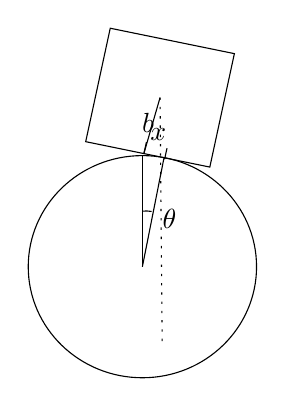
\begin{tikzpicture}[x=0.75pt,y=0.75pt,yscale=-0.8,xscale=0.8]
%uncomment if require: \path (0,300); %set diagram left start at 0, and has height of 300

%Shape: Rectangle [id:dp019264018452000542] 
\draw   (291.39,79) -- (366.15,94.3) -- (351.36,162.62) -- (276.61,147.32) -- cycle ;
%Shape: Ellipse [id:dp14150194314975284] 
\draw   (242,222.61) .. controls (242,185.66) and (272.78,155.71) .. (310.75,155.71) .. controls (348.72,155.71) and (379.5,185.66) .. (379.5,222.61) .. controls (379.5,259.55) and (348.72,289.5) .. (310.75,289.5) .. controls (272.78,289.5) and (242,259.55) .. (242,222.61) -- cycle ;
%Straight Lines [id:da998595113137927] 
\draw    (310.75,155.71) -- (310.75,222.61) ;
%Straight Lines [id:da07591077835295956] 
\draw    (323.78,157) -- (310.75,222.61) ;
%Straight Lines [id:da07451167500757727] 
\draw    (311.71,154.23) -- (313.17,147.58) ;
%Straight Lines [id:da7468603419553995] 
\draw    (324.11,157.93) -- (325.57,151.27) ;
%Shape: Arc [id:dp6044724799815564] 
\draw  [draw opacity=0] (310.67,189.17) .. controls (312.51,188.98) and (314.39,189.03) .. (316.29,189.34) -- (312.84,211.24) -- cycle ; \draw   (310.67,189.17) .. controls (312.51,188.98) and (314.39,189.03) .. (316.29,189.34) ;  
%Straight Lines [id:da9678606844801586] 
\draw  [dash pattern={on 0.84pt off 2.51pt}]  (321.38,120.81) -- (322.68,269.6) ;
%Straight Lines [id:da8736829885602427] 
\draw    (321.38,120.81) -- (311.71,154.23) ;

% Text Node
\draw (321.32,186.17) node [anchor=north west][inner sep=0.75pt]    {$\theta $};
% Text Node
\draw (314.03,138.12) node [anchor=north west][inner sep=0.75pt]    {$x$};
% Text Node
\draw (309,128.4) node [anchor=north west][inner sep=0.75pt]    {$b$};


\end{tikzpicture}
    \end{center}
The dotted line needs to be on the left side of the contact point. By observing the picture, we can get: (1) If $b<r$, then it is stable. (2) If $b>r$, then it is unstable.  
\end{problem}
\begin{problem}[The electric potential of an electric dipole]
    \begin{equation}
        U=\frac{e}{4\pi \varepsilon_0}\left(\frac{1}{\sqrt{R^2+\frac{r}{2}^2-rR\cos(\theta)}}-\frac{1}{\sqrt{R^2+\frac{r}{2}^2+rR\cos(\theta)}}\right).
    \end{equation}
    \begin{equation}
        U\approx \frac{e}{4\pi \varepsilon_0R}\frac{r}{R}\cos\theta=\frac{\vec{p}\cdot\hat{R}}{4\pi\varepsilon_0 R^2}.
    \end{equation}
    \begin{center}



\tikzset{every picture/.style={line width=0.75pt}} %set default line width to 0.75pt        

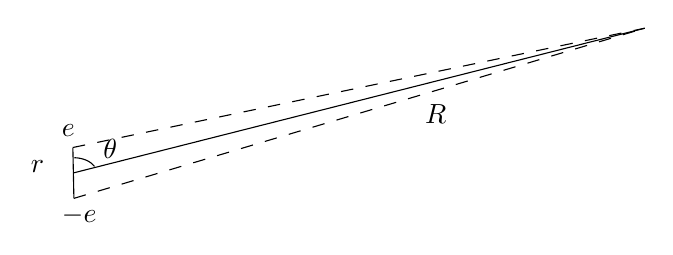
\begin{tikzpicture}[x=0.75pt,y=0.75pt,yscale=-0.7,xscale=1]
%uncomment if require: \path (0,300); %set diagram left start at 0, and has height of 300

%Straight Lines [id:da5484830962361458] 
\draw    (199.5,171) -- (200,206) ;
%Straight Lines [id:da6831505242746999] 
\draw    (199.75,188.5) -- (475.04,88.9) ;
%Straight Lines [id:da7083098046184754] 
\draw  [dash pattern={on 4.5pt off 4.5pt}]  (199.5,171) -- (475.04,88.9) ;
%Straight Lines [id:da9958680346395672] 
\draw  [dash pattern={on 4.5pt off 4.5pt}]  (200,206) -- (475.04,88.9) ;
%Shape: Arc [id:dp5093898396709098] 
\draw  [draw opacity=0] (200.26,178.01) .. controls (204.54,178.19) and (208.2,180.6) .. (209.93,184.03) -- (199.75,188.5) -- cycle ; \draw   (200.26,178.01) .. controls (204.54,178.19) and (208.2,180.6) .. (209.93,184.03) ;  

% Text Node
\draw (193,153.4) node [anchor=north west][inner sep=0.75pt]    {$e$};
% Text Node
\draw (193,209.4) node [anchor=north west][inner sep=0.75pt]    {$-e$};
% Text Node
\draw (368,139.4) node [anchor=north west][inner sep=0.75pt]    {$R$};
% Text Node
\draw (213,163.4) node [anchor=north west][inner sep=0.75pt]    {$\theta $};
% Text Node
\draw (178,178.4) node [anchor=north west][inner sep=0.75pt]    {$r$};


\end{tikzpicture}

    \end{center}
\end{problem}
\begin{problem}[The tide potential]
    (1)Let 
    \begin{equation}
        U_\mathrm{tide}(\mathbf{r})=-GMm\left(\frac{1}{\left|\mathbf{d_0+r}\right|}-\frac{1}{\left|\mathbf{d_0}\right|}\right),
    \end{equation}
    then, 
    \begin{equation}
        \mathbf{F}_\mathrm{tide}(\mathbf{r})=-\nabla U_\mathrm{tide}(\mathbf{r}).
    \end{equation}
    (2)  (We also consider the centrifugal potential energy). Since $\frac{\left|\mathbf{r}\right|}{\left|\mathbf{d_0}\right|} \ll1$,
    \begin{equation}
        \varphi_\text{tide}\approx -\frac{GMr^2}{d_0^3}\frac{3 \cos \theta^2-1}{2},
    \end{equation}
    where $r$ is the distance to the center of the earth. Sea level is a  equalpotential plain. 
    \begin{equation}
        \Delta h=\frac{3GMr^2}{2d_0^3g}.
    \end{equation}

\end{problem}
\end{document}